\chapter{The Fifth of September}

The extension provided for by the agent of Thomson \& French, at the
moment when Morrel expected it least, was to the poor shipowner so
decided a stroke of good fortune that he almost dared to believe that
fate was at length grown weary of wasting her spite upon him. The same
day he told his wife, Emmanuel, and his daughter all that had occurred;
and a ray of hope, if not of tranquillity, returned to the family.
Unfortunately, however, Morrel had not only engagements with the house
of Thomson \& French, who had shown themselves so considerate towards
him; and, as he had said, in business he had correspondents, and not
friends. When he thought the matter over, he could by no means account
for this generous conduct on the part of Thomson \& French towards him;
and could only attribute it to some such selfish argument as this: “We
had better help a man who owes us nearly 300,000 francs, and have those
300,000 francs at the end of three months than hasten his ruin, and get
only six or eight per cent of our money back again.”

Unfortunately, whether through envy or stupidity, all Morrel’s
correspondents did not take this view; and some even came to a contrary
decision. The bills signed by Morrel were presented at his office with
scrupulous exactitude, and, thanks to the delay granted by the
Englishman, were paid by Cocles with equal punctuality. Cocles thus
remained in his accustomed tranquillity. It was Morrel alone who
remembered with alarm, that if he had to repay on the 15th the 50,000
francs of M. de Boville, and on the 30th the 32,500 francs of bills,
for which, as well as the debt due to the inspector of prisons, he had
time granted, he must be a ruined man.

The opinion of all the commercial men was that, under the reverses
which had successively weighed down Morrel, it was impossible for him
to remain solvent. Great, therefore, was the astonishment when at the
end of the month, he cancelled all his obligations with his usual
punctuality. Still confidence was not restored to all minds, and the
general opinion was that the complete ruin of the unfortunate shipowner
had been postponed only until the end of the month.

The month passed, and Morrel made extraordinary efforts to get in all
his resources. Formerly his paper, at any date, was taken with
confidence, and was even in request. Morrel now tried to negotiate
bills at ninety days only, and none of the banks would give him credit.
Fortunately, Morrel had some funds coming in on which he could rely;
and, as they reached him, he found himself in a condition to meet his
engagements when the end of July came.

The agent of Thomson \& French had not been again seen at Marseilles;
the day after, or two days after his visit to Morrel, he had
disappeared; and as in that city he had had no intercourse but with the
mayor, the inspector of prisons, and M. Morrel, his departure left no
trace except in the memories of these three persons. As to the sailors
of the \textit{Pharaon}, they must have found snug berths elsewhere, for they
also had disappeared.

Captain Gaumard, recovered from his illness, had returned from Palma.
He delayed presenting himself at Morrel’s, but the owner, hearing of
his arrival, went to see him. The worthy shipowner knew, from Penelon’s
recital, of the captain’s brave conduct during the storm, and tried to
console him. He brought him also the amount of his wages, which Captain
Gaumard had not dared to apply for.

As he descended the staircase, Morrel met Penelon, who was going up.
Penelon had, it would seem, made good use of his money, for he was
newly clad. When he saw his employer, the worthy tar seemed much
embarrassed, drew on one side into the corner of the landing-place,
passed his quid from one cheek to the other, stared stupidly with his
great eyes, and only acknowledged the squeeze of the hand which Morrel
as usual gave him by a slight pressure in return. Morrel attributed
Penelon’s embarrassment to the elegance of his attire; it was evident
the good fellow had not gone to such an expense on his own account; he
was, no doubt, engaged on board some other vessel, and thus his
bashfulness arose from the fact of his not having, if we may so express
ourselves, worn mourning for the \textit{Pharaon} longer. Perhaps he had come
to tell Captain Gaumard of his good luck, and to offer him employment
from his new master.

“Worthy fellows!” said Morrel,  as he went away, “may your new master
love you as I loved you, and be more fortunate than I have been!”

\begin{figure}[ht]
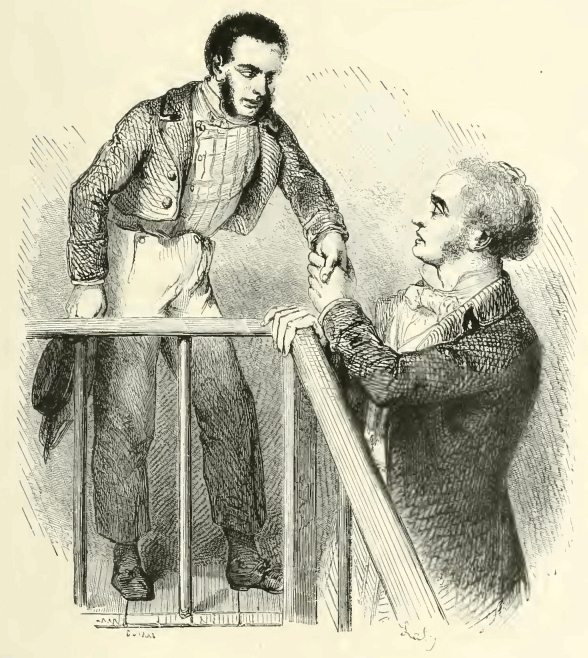
\includegraphics[width=\textwidth]{20049m.jpg}
\end{figure}

August rolled by in unceasing efforts on the part of Morrel to renew
his credit or revive the old. On the 20th of August it was known at
Marseilles that he had left town in the mailcoach, and then it was said
that the bills would go to protest at the end of the month, and that
Morrel had gone away and left his chief clerk Emmanuel, and his cashier
Cocles, to meet the creditors. But, contrary to all expectation, when
the 31st of August came, the house opened as usual, and Cocles appeared
behind the grating of the counter, examined all bills presented with
the usual scrutiny, and, from first to last, paid all with the usual
precision. There came in, moreover, two drafts which M. Morrel had
fully anticipated, and which Cocles paid as punctually as the bills
which the shipowner had accepted. All this was incomprehensible, and
then, with the tenacity peculiar to prophets of bad news, the failure
was put off until the end of September.

On the 1st, Morrel returned; he was awaited by his family with extreme
anxiety, for from this journey to Paris they hoped great things. Morrel
had thought of Danglars, who was now immensely rich, and had lain under
great obligations to Morrel in former days, since to him it was owing
that Danglars entered the service of the Spanish banker, with whom he
had laid the foundations of his vast wealth. It was said at this moment
that Danglars was worth from six to eight millions of francs, and had
unlimited credit. Danglars, then, without taking a crown from his
pocket, could save Morrel; he had but to pass his word for a loan, and
Morrel was saved. Morrel had long thought of Danglars, but had kept
away from some instinctive motive, and had delayed as long as possible
availing himself of this last resource. And Morrel was right, for he
returned home crushed by the humiliation of a refusal.

Yet, on his arrival, Morrel did not utter a complaint, or say one harsh
word. He embraced his weeping wife and daughter, pressed Emmanuel’s
hand with friendly warmth, and then going to his private room on the
second floor had sent for Cocles.

“Then,” said the two women to Emmanuel, “we are indeed ruined.”

It was agreed in a brief council held among them, that Julie should
write to her brother, who was in garrison at Nîmes, to come to them as
speedily as possible. The poor women felt instinctively that they
required all their strength to support the blow that impended. Besides,
Maximilian Morrel, though hardly two-and-twenty, had great influence
over his father.

He was a strong-minded, upright young man. At the time when he decided
on his profession his father had no desire to choose for him, but had
consulted young Maximilian’s taste. He had at once declared for a
military life, and had in consequence studied hard, passed brilliantly
through the Polytechnic School, and left it as sub-lieutenant of the
53rd of the line. For a year he had held this rank, and expected
promotion on the first vacancy. In his regiment Maximilian Morrel was
noted for his rigid observance, not only of the obligations imposed on
a soldier, but also of the duties of a man; and he thus gained the name
of “the stoic.” We need hardly say that many of those who gave him this
epithet repeated it because they had heard it, and did not even know
what it meant.

This was the young man whom his mother and sister called to their aid
to sustain them under the serious trial which they felt they would soon
have to endure. They had not mistaken the gravity of this event, for
the moment after Morrel had entered his private office with Cocles,
Julie saw the latter leave it pale, trembling, and his features
betraying the utmost consternation. She would have questioned him as he
passed by her, but the worthy creature hastened down the staircase with
unusual precipitation, and only raised his hands to heaven and
exclaimed:

“Oh, mademoiselle, mademoiselle, what a dreadful misfortune! Who could
ever have believed it!”

A moment afterwards Julie saw him go upstairs carrying two or three
heavy ledgers, a portfolio, and a bag of money.

Morrel examined the ledgers, opened the portfolio, and counted the
money. All his funds amounted to 6,000 or 8,000 francs, his bills
receivable up to the 5th to 4,000 or 5,000, which, making the best of
everything, gave him 14,000 francs to meet debts amounting to 287,500
francs. He had not even the means for making a possible settlement on
account.

However, when Morrel went down to his dinner, he appeared very calm.
This calmness was more alarming to the two women than the deepest
dejection would have been. After dinner Morrel usually went out and
used to take his coffee at the club of the Phocéens, and read the
\textit{Semaphore}; this day he did not leave the house, but returned to his
office.

As to Cocles, he seemed completely bewildered. For part of the day he
went into the courtyard, seated himself on a stone with his head bare
and exposed to the blazing sun. Emmanuel tried to comfort the women,
but his eloquence faltered. The young man was too well acquainted with
the business of the house, not to feel that a great catastrophe hung
over the Morrel family. Night came, the two women had watched, hoping
that when he left his room Morrel would come to them, but they heard
him pass before their door, and trying to conceal the noise of his
footsteps. They listened; he went into his sleeping-room, and fastened
the door inside. Madame Morrel sent her daughter to bed, and half an
hour after Julie had retired, she rose, took off her shoes, and went
stealthily along the passage, to see through the keyhole what her
husband was doing.

In the passage she saw a retreating shadow; it was Julie, who, uneasy
herself, had anticipated her mother. The young lady went towards Madame
Morrel.

“He is writing,” she said.

They had understood each other without speaking. Madame Morrel looked
again through the keyhole, Morrel was writing; but Madame Morrel
remarked, what her daughter had not observed, that her husband was
writing on stamped paper. The terrible idea that he was writing his
will flashed across her; she shuddered, and yet had not strength to
utter a word.

Next day M. Morrel seemed as calm as ever, went into his office as
usual, came to his breakfast punctually, and then, after dinner, he
placed his daughter beside him, took her head in his arms, and held her
for a long time against his bosom. In the evening, Julie told her
mother, that although he was apparently so calm, she had noticed that
her father’s heart beat violently.

The next two days passed in much the same way. On the evening of the
4th of September, M. Morrel asked his daughter for the key of his
study. Julie trembled at this request, which seemed to her of bad omen.
Why did her father ask for this key which she always kept, and which
was only taken from her in childhood as a punishment? The young girl
looked at Morrel.

“What have I done wrong, father,” she said, “that you should take this
key from me?”

“Nothing, my dear,” replied the unhappy man, the tears starting to his
eyes at this simple question,—“nothing, only I want it.”

Julie made a pretence to feel for the key. “I must have left it in my
room,” she said.

And she went out, but instead of going to her apartment she hastened to
consult Emmanuel.

“Do not give this key to your father,” said he, “and tomorrow morning,
if possible, do not quit him for a moment.”

She questioned Emmanuel, but he knew nothing, or would not say what he
knew.

During the night, between the 4th and 5th of September, Madame Morrel
remained listening for every sound, and, until three o’clock in the
morning, she heard her husband pacing the room in great agitation. It
was three o’clock when he threw himself on the bed. The mother and
daughter passed the night together. They had expected Maximilian since
the previous evening. At eight o’clock in the morning Morrel entered
their chamber. He was calm; but the agitation of the night was legible
in his pale and careworn visage. They did not dare to ask him how he
had slept. Morrel was kinder to his wife, more affectionate to his
daughter, than he had ever been. He could not cease gazing at and
kissing the sweet girl. Julie, mindful of Emmanuel’s request, was
following her father when he quitted the room, but he said to her
quickly:

“Remain with your mother, dearest.” Julie wished to accompany him. “I
wish you to do so,” said he.

This was the first time Morrel had ever so spoken, but he said it in a
tone of paternal kindness, and Julie did not dare to disobey. She
remained at the same spot standing mute and motionless. An instant
afterwards the door opened, she felt two arms encircle her, and a mouth
pressed her forehead. She looked up and uttered an exclamation of joy.

\begin{figure}[ht]
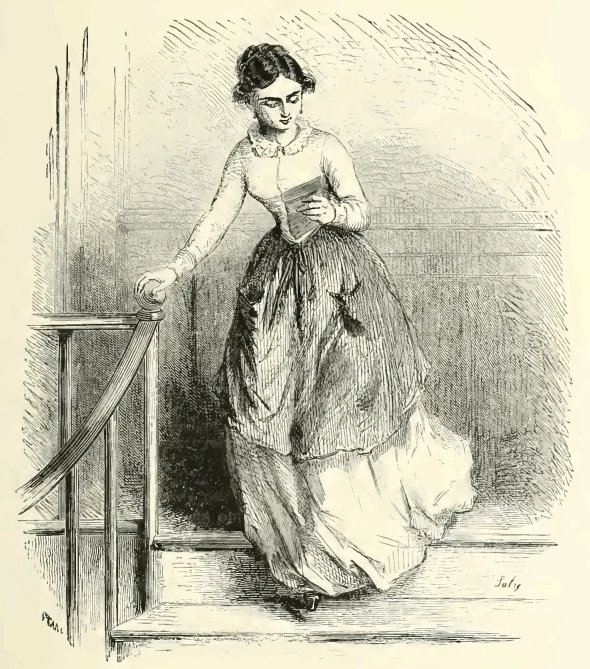
\includegraphics[width=\textwidth]{20053m.jpg}
\end{figure}

“Maximilian, my dearest brother!” she cried.

At these words Madame Morrel rose, and threw herself into her son’s
arms.

“Mother,” said the young man, looking alternately at Madame Morrel and
her daughter, “what has occurred—what has happened? Your letter has
frightened me, and I have come hither with all speed.”

“Julie,” said Madame Morrel, making a sign to the young man, “go and
tell your father that Maximilian has just arrived.”

The young lady rushed out of the apartment, but on the first step of
the staircase she found a man holding a letter in his hand.

“Are you not Mademoiselle Julie Morrel?” inquired the man, with a
strong Italian accent.

“Yes, sir,” replied Julie with hesitation; “what is your pleasure? I do
not know you.”

“Read this letter,” he said, handing it to her. Julie hesitated. “It
concerns the best interests of your father,” said the messenger.

The young girl hastily took the letter from him. She opened it quickly
and read:

“Go this moment to the Allées de Meilhan, enter the house No. 15, ask
the porter for the key of the room on the fifth floor, enter the
apartment, take from the corner of the mantelpiece a purse netted in
red silk, and give it to your father. It is important that he should
receive it before eleven o’clock. You promised to obey me implicitly.
Remember your oath.

“Sinbad the Sailor.”

The young girl uttered a joyful cry, raised her eyes, looked round to
question the messenger, but he had disappeared. She cast her eyes again
over the note to peruse it a second time, and saw there was a
postscript. She read:

“It is important that you should fulfil this mission in person and
alone. If you go accompanied by any other person, or should anyone else
go in your place, the porter will reply that he does not know anything
about it.”

This postscript decreased greatly the young girl’s happiness. Was there
nothing to fear? was there not some snare laid for her? Her innocence
had kept her in ignorance of the dangers that might assail a young girl
of her age. But there is no need to know danger in order to fear it;
indeed, it may be observed, that it is usually unknown perils that
inspire the greatest terror.

Julie hesitated, and resolved to take counsel. Yet, through a singular
impulse, it was neither to her mother nor her brother that she applied,
but to Emmanuel. She hastened down and told him what had occurred on
the day when the agent of Thomson \& French had come to her father’s,
related the scene on the staircase, repeated the promise she had made,
and showed him the letter.

“You must go, then, mademoiselle,” said Emmanuel.

“Go there?” murmured Julie.

“Yes; I will accompany you.”

“But did you not read that I must be alone?” said Julie.

“And you shall be alone,” replied the young man. “I will await you at
the corner of the Rue du Musée, and if you are so long absent as to
make me uneasy, I will hasten to rejoin you, and woe to him of whom you
shall have cause to complain to me!”

“Then, Emmanuel?” said the young girl with hesitation, “it is your
opinion that I should obey this invitation?”

“Yes. Did not the messenger say your father’s safety depended upon it?”

“But what danger threatens him, then, Emmanuel?” she asked.

Emmanuel hesitated a moment, but his desire to make Julie decide
immediately made him reply.

“Listen,” he said; “today is the 5th of September, is it not?”

“Yes.”

“Today, then, at eleven o’clock, your father has nearly three hundred
thousand francs to pay?”

“Yes, we know that.”

“Well, then,” continued Emmanuel, “we have not fifteen thousand francs
in the house.”

“What will happen then?”

“Why, if today before eleven o’clock your father has not found someone
who will come to his aid, he will be compelled at twelve o’clock to
declare himself a bankrupt.”

“Oh, come, then, come!” cried she, hastening away with the young man.

During this time, Madame Morrel had told her son everything. The young
man knew quite well that, after the succession of misfortunes which had
befallen his father, great changes had taken place in the style of
living and housekeeping; but he did not know that matters had reached
such a point. He was thunderstruck. Then, rushing hastily out of the
apartment, he ran upstairs, expecting to find his father in his study,
but he rapped there in vain.

While he was yet at the door of the study he heard the bedroom door
open, turned, and saw his father. Instead of going direct to his study,
M. Morrel had returned to his bedchamber, which he was only this moment
quitting. Morrel uttered a cry of surprise at the sight of his son, of
whose arrival he was ignorant. He remained motionless on the spot,
pressing with his left hand something he had concealed under his coat.
Maximilian sprang down the staircase, and threw his arms round his
father’s neck; but suddenly he recoiled, and placed his right hand on
Morrel’s breast.

“Father,” he exclaimed, turning pale as death, “what are you going to
do with that brace of pistols under your coat?”

“Oh, this is what I feared!” said Morrel.

“Father, father, in Heaven’s name,” exclaimed the young man, “what are
these weapons for?”

“Maximilian,” replied Morrel, looking fixedly at his son, “you are a
man, and a man of honor. Come, and I will explain to you.”

And with a firm step Morrel went up to his study, while Maximilian
followed him, trembling as he went. Morrel opened the door, and closed
it behind his son; then, crossing the anteroom, went to his desk on
which he placed the pistols, and pointed with his finger to an open
ledger. In this ledger was made out an exact balance-sheet of his
affairs. Morrel had to pay, within half an hour, 287,500 francs. All he
possessed was 15,257 francs.

“Read!” said Morrel.

The young man was overwhelmed as he read. Morrel said not a word. What
could he say? What need he add to such a desperate proof in figures?

“And have you done all that is possible, father, to meet this
disastrous result?” asked the young man, after a moment’s pause.

“I have,” replied Morrel.

“You have no money coming in on which you can rely?”

“None.”

“You have exhausted every resource?”

“All.”

“And in half an hour,” said Maximilian in a gloomy voice, “our name is
dishonored!”

“Blood washes out dishonor,” said Morrel.

“You are right, father; I understand you.” Then extending his hand
towards one of the pistols, he said, “There is one for you and one for
me—thanks!”

Morrel caught his hand. “Your mother—your sister! Who will support
them?”

A shudder ran through the young man’s frame. “Father,” he said, “do you
reflect that you are bidding me to live?”

“Yes, I do so bid you,” answered Morrel, “it is your duty. You have a
calm, strong mind, Maximilian. Maximilian, you are no ordinary man. I
make no requests or commands; I only ask you to examine my position as
if it were your own, and then judge for yourself.”

The young man reflected for a moment, then an expression of sublime
resignation appeared in his eyes, and with a slow and sad gesture he
took off his two epaulets, the insignia of his rank.

“Be it so, then, my father,” he said, extending his hand to Morrel,
“die in peace, my father; I will live.”

Morrel was about to cast himself on his knees before his son, but
Maximilian caught him in his arms, and those two noble hearts were
pressed against each other for a moment.

“You know it is not my fault,” said Morrel.

\begin{figure}[ht]
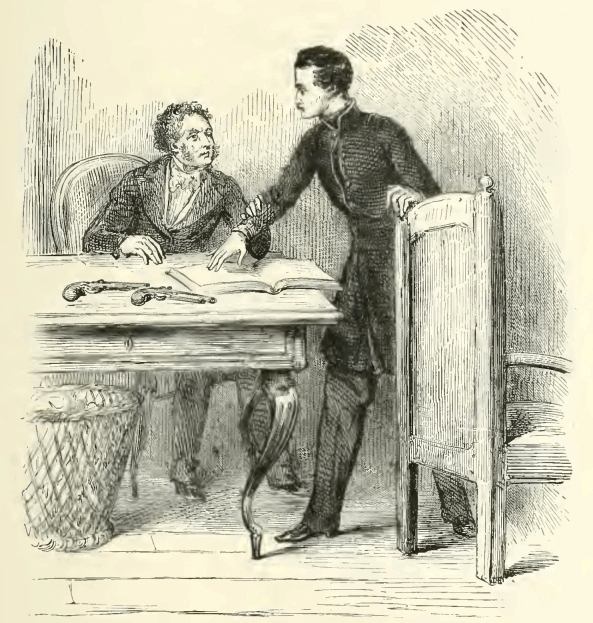
\includegraphics[width=\textwidth]{20057m.jpg}
\end{figure}

Maximilian smiled. “I know, father, you are the most honorable man I
have ever known.”

“Good, my son. And now there is no more to be said; go and rejoin your
mother and sister.”

“My father,” said the young man, bending his knee, “bless me!” Morrel
took the head of his son between his two hands, drew him forward, and
kissing his forehead several times said:

“Oh, yes, yes, I bless you in my own name, and in the name of three
generations of irreproachable men, who say through me, ‘The edifice
which misfortune has destroyed, Providence may build up again.’ On
seeing me die such a death, the most inexorable will have pity on you.
To you, perhaps, they will accord the time they have refused to me.
Then do your best to keep our name free from dishonor. Go to work,
labor, young man, struggle ardently and courageously; live, yourself,
your mother and sister, with the most rigid economy, so that from day
to day the property of those whom I leave in your hands may augment and
fructify. Reflect how glorious a day it will be, how grand, how solemn,
that day of complete restoration, on which you will say in this very
office, ‘My father died because he could not do what I have this day
done; but he died calmly and peaceably, because in dying he knew what I
should do.’”

“My father, my father!” cried the young man, “why should you not live?”

“If I live, all would be changed; if I live, interest would be
converted into doubt, pity into hostility; if I live I am only a man
who has broken his word, failed in his engagements—in fact, only a
bankrupt. If, on the contrary, I die, remember, Maximilian, my corpse
is that of an honest but unfortunate man. Living, my best friends would
avoid my house; dead, all Marseilles will follow me in tears to my last
home. Living, you would feel shame at my name; dead, you may raise your
head and say, ‘I am the son of him you killed, because, for the first
time, he has been compelled to break his word.’”

The young man uttered a groan, but appeared resigned.

“And now,” said Morrel, “leave me alone, and endeavor to keep your
mother and sister away.”

“Will you not see my sister once more?” asked Maximilian. A last but
final hope was concealed by the young man in the effect of this
interview, and therefore he had suggested it. Morrel shook his head. “I
saw her this morning, and bade her adieu.”

“Have you no particular commands to leave with me, my father?” inquired
Maximilian in a faltering voice.

“Yes; my son, and a sacred command.”

“Say it, my father.”

“The house of Thomson \& French is the only one who, from humanity, or,
it may be, selfishness—it is not for me to read men’s hearts—has had
any pity for me. Its agent, who will in ten minutes present himself to
receive the amount of a bill of 287,500 francs, I will not say granted,
but offered me three months. Let this house be the first repaid, my
son, and respect this man.”

“Father, I will,” said Maximilian.

“And now, once more, adieu,” said Morrel. “Go, leave me; I would be
alone. You will find my will in the secretaire in my bedroom.”

The young man remained standing and motionless, having but the force of
will and not the power of execution.

“Hear me, Maximilian,” said his father. “Suppose I were a soldier like
you, and ordered to carry a certain redoubt, and you knew I must be
killed in the assault, would you not say to me, as you said just now,
‘Go, father; for you are dishonored by delay, and death is preferable
to shame!’”

“Yes, yes,” said the young man, “yes;” and once again embracing his
father with convulsive pressure, he said, “Be it so, my father.”

And he rushed out of the study. When his son had left him, Morrel
remained an instant standing with his eyes fixed on the door; then
putting forth his arm, he pulled the bell. After a moment’s interval,
Cocles appeared.

It was no longer the same man—the fearful revelations of the three last
days had crushed him. This thought—the house of Morrel is about to stop
payment—bent him to the earth more than twenty years would otherwise
have done.

“My worthy Cocles,” said Morrel in a tone impossible to describe, “do
you remain in the antechamber. When the gentleman who came three months
ago—the agent of Thomson \& French—arrives, announce his arrival to me.”

Cocles made no reply; he made a sign with his head, went into the
anteroom, and seated himself. Morrel fell back in his chair, his eyes
fixed on the clock; there were seven minutes left, that was all. The
hand moved on with incredible rapidity, he seemed to see its motion.

What passed in the mind of this man at the supreme moment of his agony
cannot be told in words. He was still comparatively young, he was
surrounded by the loving care of a devoted family, but he had convinced
himself by a course of reasoning, illogical perhaps, yet certainly
plausible, that he must separate himself from all he held dear in the
world, even life itself. To form the slightest idea of his feelings,
one must have seen his face with its expression of enforced resignation
and its tear-moistened eyes raised to heaven. The minute hand moved on.
The pistols were loaded; he stretched forth his hand, took one up, and
murmured his daughter’s name. Then he laid it down, seized his pen, and
wrote a few words. It seemed to him as if he had not taken a sufficient
farewell of his beloved daughter. Then he turned again to the clock,
counting time now not by minutes, but by seconds.

He took up the deadly weapon again, his lips parted and his eyes fixed
on the clock, and then shuddered at the click of the trigger as he
cocked the pistol. At this moment of mortal anguish the cold sweat came
forth upon his brow, a pang stronger than death clutched at his
heart-strings. He heard the door of the staircase creak on its
hinges—the clock gave its warning to strike eleven—the door of his
study opened. Morrel did not turn round—he expected these words of
Cocles, “The agent of Thomson \& French.”

He placed the muzzle of the pistol between his teeth. Suddenly he heard
a cry—it was his daughter’s voice. He turned and saw Julie. The pistol
fell from his hands.

“My father!” cried the young girl, out of breath, and half dead with
joy—“saved, you are saved!” And she threw herself into his arms,
holding in her extended hand a red, netted silk purse.

\begin{figure}[h]
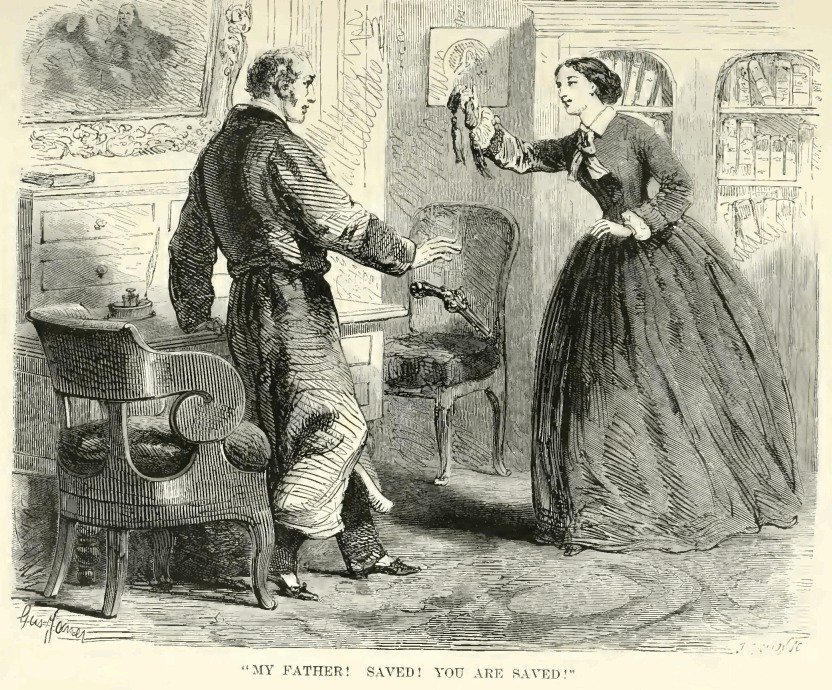
\includegraphics[width=\textwidth]{20061m.jpg}
\end{figure}

“Saved, my child!” said Morrel; “what do you mean?”

“Yes, saved—saved! See, see!” said the young girl.

Morrel took the purse, and started as he did so, for a vague
remembrance reminded him that it once belonged to himself. At one end
was the receipted bill for the 287,000 francs, and at the other was a
diamond as large as a hazel-nut, with these words on a small slip of
parchment: \textit{Julie’s Dowry}.

Morrel passed his hand over his brow; it seemed to him a dream. At this
moment the clock struck eleven. He felt as if each stroke of the hammer
fell upon his heart.

“Explain, my child,” he said, “Explain, my child,” he said,
“explain—where did you find this purse?”

“In a house in the Allées de Meilhan, No. 15, on the corner of a
mantelpiece in a small room on the fifth floor.”

“But,” cried Morrel, “this purse is not yours!” Julie handed to her
father the letter she had received in the morning.

“And did you go alone?” asked Morrel, after he had read it.

“Emmanuel accompanied me, father. He was to have waited for me at the
corner of the Rue du Musée, but, strange to say, he was not there when
I returned.”

“Monsieur Morrel!” exclaimed a voice on the stairs; “Monsieur Morrel!”

“It is his voice!” said Julie. At this moment Emmanuel entered, his
countenance full of animation and joy.

“The \textit{Pharaon}!” he cried; “the \textit{Pharaon}!”

“What!—what!—the \textit{Pharaon}! Are you mad, Emmanuel? You know the vessel
is lost.”

“The \textit{Pharaon}, sir—they signal the \textit{Pharaon}! The \textit{Pharaon} is
entering the harbor!”

Morrel fell back in his chair, his strength was failing him; his
understanding weakened by such events, refused to comprehend such
incredible, unheard-of, fabulous facts. But his son came in.

“Father,” cried Maximilian, “how could you say the \textit{Pharaon} was lost?
The lookout has signalled her, and they say she is now coming into
port.”

\begin{figure}[ht]
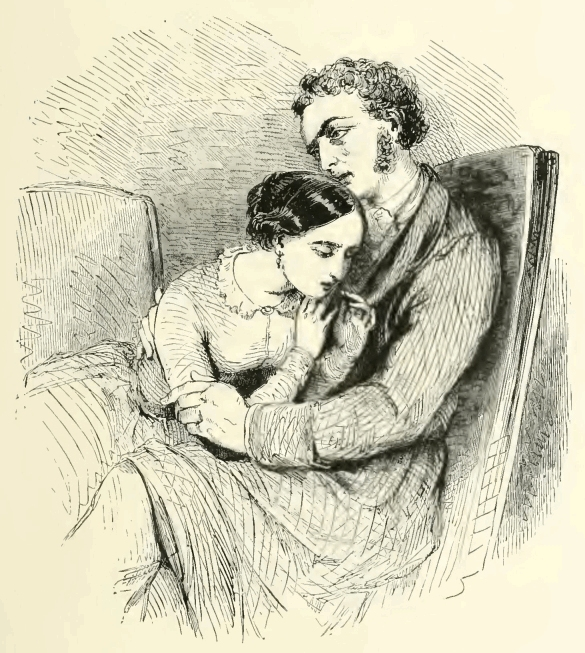
\includegraphics[width=\textwidth]{20063m.jpg}
\end{figure}

“My dear friends,” said Morrel, “if this be so, it must be a miracle of
heaven! Impossible, impossible!”

But what was real and not less incredible was the purse he held in his
hand, the acceptance receipted—the splendid diamond.

“Ah, sir,” exclaimed Cocles, “what can it mean?—the \textit{Pharaon}?”

“Come, dear ones,” said Morrel, rising from his seat, “let us go and
see, and Heaven have pity upon us if it be false intelligence!”

They all went out, and on the stairs met Madame Morrel, who had been
afraid to go up into the study. In a moment they were at the Canebière.
There was a crowd on the pier. All the crowd gave way before Morrel.
“The \textit{Pharaon}! the \textit{Pharaon}!” said every voice.

And, wonderful to see, in front of the tower of Saint-Jean, was a ship
bearing on her stern these words, printed in white letters, “The
\textit{Pharaon}, Morrel \& Son, of Marseilles.” She was the exact duplicate of
the other \textit{Pharaon}, and loaded, as that had been, with cochineal and
indigo. She cast anchor, clued up sails, and on the deck was Captain
Gaumard giving orders, and good old Penelon making signals to M.
Morrel. To doubt any longer was impossible; there was the evidence of
the senses, and ten thousand persons who came to corroborate the
testimony.

As Morrel and his son embraced on the pier-head, in the presence and
amid the applause of the whole city witnessing this event, a man, with
his face half-covered by a black beard, and who, concealed behind the
sentry-box, watched the scene with delight, uttered these words in a
low tone:

“Be happy, noble heart, be blessed for all the good thou hast done and
wilt do hereafter, and let my gratitude remain in obscurity like your
good deeds.”

\begin{figure}[ht]
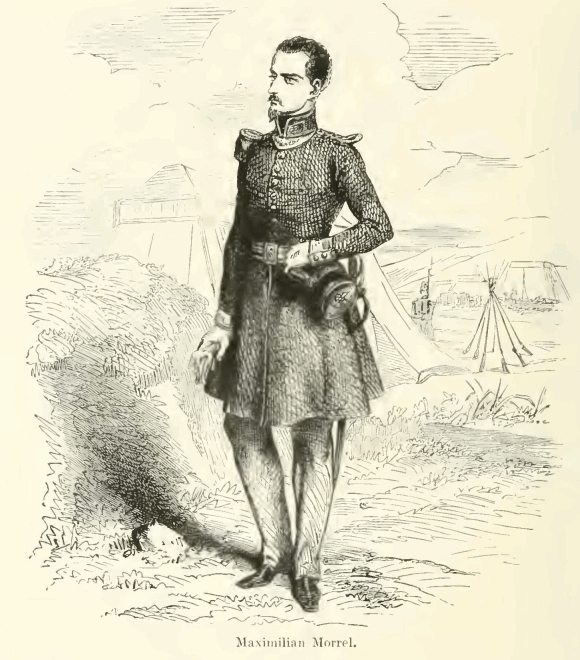
\includegraphics[width=\textwidth]{20064m.jpg}
\end{figure}

And with a smile expressive of supreme content, he left his
hiding-place, and without being observed, descended one of the flights
of steps provided for debarkation, and hailing three times, shouted
“Jacopo, Jacopo, Jacopo!”

Then a launch came to shore, took him on board, and conveyed him to a
yacht splendidly fitted up, on whose deck he sprung with the activity
of a sailor; thence he once again looked towards Morrel, who, weeping
with joy, was shaking hands most cordially with all the crowd around
him, and thanking with a look the unknown benefactor whom he seemed to
be seeking in the skies.

“And now,” said the unknown, “farewell kindness, humanity, and
gratitude! Farewell to all the feelings that expand the heart! I have
been Heaven’s substitute to recompense the good—now the god of
vengeance yields to me his power to punish the wicked!”

At these words he gave a signal, and, as if only awaiting this signal,
the yacht instantly put out to sea.
